\documentclass[12pt]{article}
\usepackage{kyradefaults}
\addbibresource{references.bib}

\title{\textbf{All Aboard? Causal Evidence on the Labor-Market Effects of New Rail Stations}}
\author{Kyra Sadovi%
  \thanks{E-Mail: \texttt{ksadovi@uchicago.edu}}}
\affil{Harris School of Public Policy, University of Chicago}
\date{}

\begin{document}
\maketitle
\thispagestyle{empty}
 \begin{abstract}
 \noindent In this proposal, I set out the framing for a paper which estimates the causal effect of new rail station access on nearby residents' labor-market outcomes, focusing on worker flows and income. New stations may improve outcomes through three mechanisms: more reliable commuting to existing jobs, expanded job-search radius across the metro area, and broader referral networks. Identifying these effects is complicated by non-random station placement, residential sorting, and anticipatory adjustment. I address these challenges by exploiting quasi-random variation in station opening timing generated by construction delays, embedding the design in a stacked difference-in-differences framework that yields robust event-study estimates under staggered adoption. A novel dataset of U.S. rail projects since 2000 links planned opening dates — drawn from Draft Environmental Impact Statements — to realized opening dates and station geographies. Labor-market outcomes come from Census LODES, and transit exposure is measured via walking-time isochrones computed using the \texttt{r5r} routing package.
 \end{abstract}
\newpage 
\section{Introduction}
As cities across the world continue to expand in the midst of the ongoing process of urbanization, much of the conversation around infrastructure, resource allocation, and expanded networks comes down to how to ease congestion while getting workers and residents from point A to point B. In the context of the United States, urban public transportation has been dramatically underfunded for decades in most cities --- the justification being that such an investment would be a waste of resources based on the assumption that public transit's take-up in the U.S. is too low. In this paper, I will demonstrate that worker flows into and out of neighborhoods which receive new public transit stations shift as a causal result of exposure to these transit networks. This evidence could serve as a first stage to measure the downstream network effects of transit --- increased worker flows indicate more (and shifted) interactions between new residents and new workers in a given neighborhood, leading to more information exchange, referral effects, and potential welfare gains as a result. 

For the purpose of this flow analysis, I propose using U.S. light rail project construction delays as a plausibly exogenous source of variation for an adjusted staggered difference-in-differences approach, thereby isolating the effect of gaining physical access to a transit station. 

It is important to emphasize that I am interested in the effects of gaining physical access to a transit system on residents' outcomes rather than the overall, multifaceted impact of transit. The reason I make this distinction is because my delay setup intentionally differences out all anticipation effects. As \textcite{mcmillenReactionHousePrices2004} find in their paper on the opening of Chicago's Orange Line, non-labor economic indicators such as house prices can respond to the announcement of a planned station up to six years in advance of the station actually opening. While this is an interesting research question in and of itself, it is not the subject of this paper. 

Decreased commuting costs impact labor market outcomes through three distinct (though related) mechanisms: more reliable means of commuting make it more likely that a worker retains their current employment \parencite{sanchezConnectionPublicTransit1999}; an expanded plausible job-search radius within a given metropolitan area \parencite{perezUrbanTransitInfrastructure2022, donaldsonRailroadsAmericanEconomic2016}; and broader referral networks \parencite{patacchini_referral_fx, kimSpatialInteractions2023}. My model setup is specifically designed to isolate transit's effects on residents via these mechanisms --- in short, to measure the effect of gaining access to a system rather than the effect of being chosen for a transit station. Comparing tracts with stations to those which are soon-to-receive stations allows me to estimate this effect, essentially the average treatment effect on the treated (with treatment here being receipt of a station). 

While this is a question that has been the subject of much of the transit economics literature (see \textcite{tsivanidisEvaluatingImpactUrban2026}, \textcite{tyndall_airports}, and \textcite{Gupta} as just a few examples), my setting and specific posture offers the potential to isolate transit impacts on agents as residents rather than as workers --- effectively, measuring the other node of the commute to work relative to \citeauthor{tsivanidisEvaluatingImpactUrban2026} or \citeauthor{perezUrbanTransitInfrastructure2022}. But even relative to \citeauthor{tyndall_airports}'s work using airport lines as an albeit ingenious instrument to measure labor market outcomes, my proposal offers the potential to expand on his case-study setup and make the results generalizable to transit projects across the country. 

\citeauthor{perezUrbanTransitInfrastructure2022} offer a similar analysis of transit to the current setting, though from the ``opposite node.'' One can envision the commuting problem as a binodal one, with one node being a person's residence and the other being their place of work. Much of the focus of the transit literature is, rightly so, centered on the place of work. I argue that there is just as much welfare gain that comes from the residential node: neighbors, peers, and children will interact in different ways when their networks shift and expand. For example, \cite{patacchini_referral_fx} find that as social networks expand, labor market referral effects increase dramatically. In the realm of financial literacy, \cite{frisanchoSpilloverEffectsFinancial2023} demonstrate how the effects of financial education for children spill over to parents and parents' peers. 

While these flow conclusions are useful in a limited sense, their largest advantage is that they support further research on the residential impact of transit. Just as \cite{perezUrbanTransitInfrastructure2022}, \cite{almagro_amenities}, \cite{tsivanidisEvaluatingImpactUrban2022}, and more demonstrate, welfare analyses of transit shocks are directly relevant to measuring how cities should most effectively be structured. I argue that this analysis should focus not just on the place of work, but the place of residence. As such, treating each station node as a residential locus, my next steps in this project would be to analyze the welfare effects of connecting residential locations to the urban transport network. In this paper, construction delays are my instrument for identifying the causal effect of transit on worker flows. But in next steps, increased worker flows are really the instrument for identifying social shocks as an avenue of financial education.  \hl{talk about expanded data access, a spatial model TK, and residential welfare gains.}

\hl{Have a more concerted section placing this in the context of the literature. Right now I'm justifying why this works, I think I need}

\section{Data and Background}
If I were given carte blanche to measure the labor market or welfare impacts of public transit, I would have to completely randomize resident locations, workplace locations, and resident demographics as well as station location characteristics in order to isolate transit's impact from the many sources of endogeneity characteristic of analyses like this. As I am not afforded that convenience, I contest that my delay setup does a good job of isolating these effects. 

As I'll discuss more in section \ref{sec:data}, I have collected data on construction and environmental impact records of new transit projects in urban American cities in the last twenty years. The reason I've focused on the United States is because of the country's particular attitude toward public transportation and increasing trends of urbanization and congestion \parencite{roseTrafficCongestionHits2025, fhwa2026ucr}. Whether or not Americans are reticent to use public transit or are simply not afforded the opportunity to do so is the underlying debate among public policymakers deciding whether to invest more funds in public transit projects. Rejecting the null that Americans do not change their behavior when given access to a new transit station would support the claim that increased funding for public transit would increase residents' welfare and employment outcomes. While the same question could be asked in other settings (and has), those results are often considered not generalizable to the American worker. This paper could answer that concern directly. 

\subsection{Data \& Feasibility}\label{sec:data}
There are two sources of data I need to complete this analysis: information on public transit construction projects, and time-series data on labor-market outcomes at least at the Census tract level (the more granular, the better). 

\subsubsection{Delay Data}
The transit data that needs to be collected is all new station locations in the last 20 years; their opened dates; their announcement dates; and their projected opened dates. I have collected data on 230 stations so far, 94 of which have been opened. I started this collection based on the dataset compiled by \textcite{levy_2025_9wnjp-kez15}, but as I started filling in the delay information system by system I noticed a number of overlooked projects. I've since been updating this as I go. Further, allowing for some time to pass for more recent stations to come online will benefit my number of observations greatly. I discuss this below in my MDE discussion. 

For each transit project, I identify the Draft Environmental Impact Statement (DEIS) or equivalent document that first evaluated the station alignment and locations ultimately built, recording its publication or Federal Register notice date as \texttt{initial\_DEIS\_date}. Where a project's alignment changed substantially after the original environmental review — as with San Francisco's Central Subway — I use the first supplemental draft document that evaluated the as-built alignment rather than the original DEIS. To derive \texttt{initial\_expected\_open\_date}, I extract the earliest specific projected completion date from the DEIS, FEIS, or contemporary sources, applying construction durations sequentially where no calendar date is explicitly stated. This approach ensures that both reference dates are tied directly to verifiable primary sources and reflect the earliest documented planning assumptions for each project's current configuration.

\subsubsection{Worker Flow Data}
In an ideal world, it would be most useful to have longitudinal panel data on employment outcomes at the resident level over time. I would need information on where the person lives and where they work --- the type of data which is available in the confidential LEHD Origin-Destination Employment Statistics (LODES) data \parencite{census_lodes}. From here, I would essentially create a ``catchment'' area around each station, identifying all people who fall within this area. An example of such a catchment area can be seen in figure \ref{fig:catchment}. For each station, I define three catchment isochrones at the 5-, 15-, and 30-minute levels. An isochrone is a boundary drawn around a point such that every location on the boundary takes the same amount of time to reach from that point. In the context of the current phase of my project, a 5-minute isochrone around a transit station captures all census tracts within a 5-minute walk of that station. These isochrones are drawn using the \texttt{r5r} package designed by \textcite{r5r}. 

Being constrained to public data is not a fundamental challenge, however: the public LODES data is available at fairly granular geographic levels, and given the amount of variation available from the transit data I have it shouldn't be an issue for at least initial treatment effect estimates. However, there's a larger problem with LODES: data reporting discrepancies. As \textcite{abrahamExploringDifferencesEmployment2013} demonstrate, employers often misreport their employees' places of work. LODES and other Census data repositories tend to source their employment data from employers themselves rather than workers; as a result, employer-side data reporting issues arise rather than worker discrepancies. Employers, consequently, will either mistakenly or intentionally (for reporting burden reasons, most frequently) report that their employees' physical place of work is the headquarters site rather than their actual physical office. This poses fundamental data credibility issues for the LODES-sourced worker flow data. 

As a result, my ideal worker information data would be sourced from \textcite{infogroup_residential}, which is available via the Becker Friedman Institute. These data solve the granularity issue and would enable me to get microeconomic estimates of treatment effects based on a number of rich demographic data rather than tract aggregates. While it does not solve the issue of employer location misreporting, the fact that it can be matched with external data gives rise to potentially more credible data in the future. I discuss these data concerns further in section \ref{subsubsec:incumbents}.

\section{Model}\label{sec:design}
The parameter of interest is the average treatment effect on the treated (ATT) of a new transit station opening on surrounding labor markets --- specifically, the causal effect on log worker inflows and outflows to census tracts that actually receive a station. I also seek to recover the dynamic version of this parameter: how the effect evolves over time relative to actual station opening, which requires identifying a separate coefficient for each period $k$ in event time.

\subsection{Time Indexes}\label{subsec:time_index}
Identification relies on the conditional exogeneity of construction delays. In order to use this instrument, I have to create two different time indexes, $j$ and $k$. Let 
\begin{equation}\label{eq:proj_time}
    j = \text{census year} - \text{initial expected open year}
\end{equation} 
denote project time --- the year relative to when a station was originally projected to open, as recorded in the Draft Environmental Impact Statement. The key assumption is that, conditional on project time $j$ and census tract fixed effects, the timing of actual station opening is as-good-as-random:
$$\mathbb{E}[Y_{it}(0) \mid \text{open}_{it},\, j_{it},\, \text{tract}_i] = \mathbb{E}[Y_{it}(0) \mid j_{it},\, \text{tract}_i].$$
This is motivated by the institutional observation that construction delays are driven primarily by engineering complications, contracting failures, and subsurface geology rather than by anticipatory changes in neighborhood economic conditions. Critically, initial projected opening dates are fixed at the DEIS or FEIS stage --- years before construction begins --- meaning they predate any local economic response to the project.

The second time index, $k$, can be understood as event time --- the year relative to when the station actually opened. So I define $k$ as

\begin{equation}\label{eq:event_time}
    k = \text{census year}-\text{actual open year}
\end{equation}
\subsection{A Defense of the Delay Instrument}
Among the identifying assumptions, I view conditional parallel trends as the most credible, since project-time fixed effects absorb the systematic relationship between neighborhood characteristics and project schedules. The conditional exogeneity of delays is somewhat less certain, as political economy considerations could cause stations in economically distressed areas to face longer delays, though tract fixed effects mitigate this concern. The least credible assumption is SUTVA: tracts near multiple stations, or near both an opened and a delayed station, could experience spillovers that contaminate the control group.

The institutional features most important for identification are (1) that initial projected opening dates are fixed in federal planning documents well before construction begins, making them plausibly orthogonal to subsequent local trends, and (2) that the proximate causes of delay --- underground obstructions, cost overruns, contractor disputes --- are unrelated to the economic trajectory of adjacent neighborhoods. I provide several pieces of evidence in support of these features. Figure \ref{fig:balance_covariates} reports covariate balance across groups defined by delay length: point estimates are small relative to their confidence intervals and centered near zero across all six pre-treatment tract characteristics, consistent with delays being orthogonal to baseline neighborhood conditions. Figure \ref{fig:delay_income} plots construction delay against tract-level median household income and reveals no discernible relationship, further supporting the claim that longer delays are not concentrated in systematically richer or poorer neighborhoods. Figure \ref{fig:balance_regression} presents coefficients from a regression of delay length on pre-treatment tract characteristics; none of the covariates are precisely estimated and all confidence intervals include zero. Figures \ref{fig:delay_state} and \ref{fig:delay_system} additionally document that delay variation is distributed across states and transit systems rather than being driven by a single agency or geography, reducing concern that unobserved system-level confounders are driving the results.

The first-pass specification is a static two-way fixed effects regression,

$$\log Y_{ij} = \alpha_i + \delta_j + \beta\, \mathbf{1}[\text{census year} \geq \text{open year}_i] + \mathbf{X}_{ij}'\gamma + \varepsilon_{ij}$$
The indexes are defined such that $i$ is Census tracts, $j$ is project-time (equation \ref{eq:proj_time}). So $\alpha_i$ are census tract fixed effects, $\delta_j$ are project-time fixed effects, and $\mathbf{X}_{ij}'\gamma$ are controls. The reason each Census tract has an open date is because for each station in my data I've identified a set of tracts within each of the aforementioned three isochrones. I treat all station events as tract events, since changes to the station schedule define the treatment of a tract. 

For dynamic effects, I estimate an event study with a full set of dummies for $k$ (equation \ref{eq:event_time}), normalizing to $k = -1$. Standard errors are clustered at the census tract level throughout, with two-way clustering at the tract and transit-system level as a robustness check. Here, $l$ refers to the isochrone.

$$\log Y_{ij} = \delta_j + \sum_{k \neq -1} \sum_l \beta_{kl} \cdot \mathbf{1}[K_{ij} = k] \cdot \mathbf{1}[L_i = l] + \mathbf{X}_{ij}'\gamma + \varepsilon_{ij}$$

Preliminary results are encouraging. Figure \ref{fig:es_inflows} presents the event study for log inflows. Pre-opening coefficients are flat and statistically indistinguishable from zero in the years immediately preceding opening, consistent with the parallel trends assumption. Following station opening, inflows rise steadily and persistently, reaching approximately one log point above baseline by ten years post-opening. The growing magnitude of the effect over time suggests that transit access reshapes residential sorting gradually, as workers update location decisions in response to improved commute options, rather than producing a one-time discrete jump at opening.

\section{Results}

\section{Planning}
\subsection{Timeline and Next Steps}
My timeline for this project is fairly short because I've been working on it for the better part of the last year. I hope to have most of this wrapped up by the end of the summer, as I am aiming to use this for my second-year paper requirement at Harris. Because this project was designed to use publicly accessible data and data I collected myself, I don't need any funding to finalize this. However, now that I've compiled all of the information on station delays and taken a first pass at at analysis, I want to get in touch with the Transit Costs Project to alert them to some stations they failed to collect. I think the construction data I've collected might be of interest to them, and potential collaborations keeping station data up-to-date both benefits their mission and would provide more station-opening observations which would make my results more robust (see discussion about concerns below). 

\subsection{Concerns}
\subsubsection{Limited Observations}\label{subsubsec:lim_obs}
While I do have a relatively large number of station openings (92 stations at the moment), I'm concerned about lack of variation in delay observations. For example, a transit system may have three new stations planned, all of which are affected by the same delay. I've plotted the histogram of station delays by transit system in figure \ref{fig:delay_hist}, constraining to systems with multiple stations. Each of these systems has at least one spike which outstrips the other stations; some, like the San Francisco Municipal Railway and Bay Area Rapit Transit, exhibit exactly my concern here: while they provide five and two stations respectively, they really only contribute one instance of variation each. 

I need to think a bit more about how much of a danger this poses to my analysis. I think my concern is twofold: both the within-system delay clumping, and the system-level clumping of station openings. For example, Sound Transit has 38 new stations, while Miami only has one. Measuring the labor-market impact of being brought into a network that is robust versus weak is substantially different. For this reason, I've been considering creating some kind of measure of the strength of a transit system (either number of existing stations, ridership per capita, or something else similar) --- but in order for this or any other controls to be useful, I simply need more observations. 

\subsubsection{SUTVA Violations and Spillovers}
The previous discussion of lack of observations directly speaks to SUTVA violations --- take the example of a one-station system. Residents in the catchment area of that new station remain unaffected by any other station openings because they do not exist. Residents in the catchment area of a station in a system with many other station openings, however, are affected by the other openings. Worse, take the example of four consecutive stations (pictured in abstract below). The green dots denote new stations just opened; red dot is station not yet opened; black dot is a preexisting station. My setup uses people in the station B catchment area as controls, and people in the station A and C catchment areas as treated observations. 

\begin{figure}[H]
    \centering
    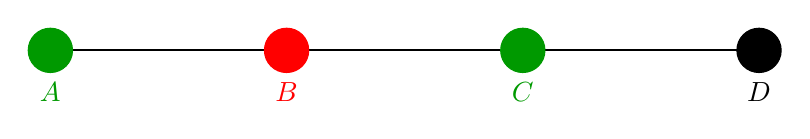
\begin{tikzpicture}
        \draw[thick] (0,0) -- (9,0);
        \filldraw[green!60!black] (0,0) circle (8pt) node[below=8pt] {$A$};
        \filldraw[red]            (3,0) circle (8pt) node[below=8pt] {$B$};
        \filldraw[green!60!black] (6,0) circle (8pt) node[below=8pt] {$C$};
        \filldraw[black]          (9,0) circle (8pt) node[below=8pt] {$D$};
    \end{tikzpicture}
    \caption{Multiple Station Example}
\end{figure}
But this is concerning for multiple reasons. First, the people treated by station C in the largest isochrone (so on the outskirts of the catchment area) may have a very different treatment effect than those in the outskirts of station A because they may be equidistant or closer to being ambivalent between stations C and D. But worse is the fact that depending on the distance between station B and other active stations, people in station B's catchment radius may already be opting into the other two radii. If this were happening across all not-yet-opened stations' catchment radii, I wouldn't be as concerned. But I think I need to start to accomodate for intensity of treatment across all of these isochrones. This would alleviate both some of the SUTVA concerns and potentially do more to be more specific about what my treatment is capturing. 

\subsubsection{Bigger picture: incumbent versus incoming residents}\label{subsubsec:incumbents}
Since I am using publicly accessible data, I have no choice but to take as given the labor market variables available at the census tract level. However, I am very limited in my ability currently to account for changes in census tract composition. In an ideal world, I would be able to identify when they moved into an area and whether they are a homeowner or a renter. For now, I remain agnostic about the composition effects of new transit, and --- beyond the effects I'm trying to capture --- the reality of changing neighborhood compositions over time. I acknowledge that this is a blaring flaw in my analysis. 

For this reason, it would be incredibly useful to gain access to confidential LODES data or, barring that unlikely scenario, use the individual level residential Infogroup data to track movements across tracts. However, the Infogroup data (as far as I am aware) does not provide data on labor market outcomes. Without some ability to track who is entering and exiting a tract and when, I am concerned that my analysis becomes fairly muddled. 

\newpage
\printbibliography
\newpage
\section*{Appendix}\label{sec:appendix}
\subsection*{Figures}\label{subsec:figs}
\begin{figure}[H]
    \centering
    
\includegraphics[width=\linewidth]{3_output/2_figures/1_maps/1_station_geographies/LA Metro_2020.pdf}
    \caption{}
    \label{fig:catchment}
\end{figure}
\begin{figure}[H]
    \centering
    
\includegraphics[width=0.8\linewidth]{3_output/2_figures/2_delay_robustness/cross_vs_within_system_coef_plot.png}
    \caption{}\label{fig:balance_covariates}
\end{figure}
\begin{figure}[H]
    \centering
    
\includegraphics[width=0.8\linewidth]{3_output/2_figures/2_delay_robustness/delay_vs_income.png}
    \caption{}\label{fig:delay_income}
\end{figure}
\begin{figure}[H]
    \centering
    
\includegraphics[width=0.8\linewidth]{3_output/2_figures/2_delay_robustness/within_system_coef_plot.png}
    \caption{}
    \label{fig:balance_regression}
\end{figure}
\begin{figure}[H]
    \centering
    
\includegraphics[width=0.8\linewidth]{3_output/2_figures/2_delay_robustness/mean_delay_by_state.png}
    \caption{}
    \label{fig:delay_state}
\end{figure}
\begin{figure}[H]
    \centering
    
\includegraphics[width=0.8\linewidth]{3_output/2_figures/2_delay_robustness/mean_delay_by_system.png}
    \caption{}
    \label{fig:delay_system}
\end{figure}
\begin{figure}[H]
    \centering
    
\includegraphics[width=0.8\linewidth]{3_output/2_figures/2_delay_robustness/delay_hist.pdf}
    \caption{}
    \label{fig:delay_hist}
\end{figure}
\begin{figure}[H]
    \centering
    
\includegraphics[width=0.8\linewidth]{3_output/2_figures/3_reg_output_plots/inflows_es.pdf}
    \caption{}
    \label{fig:es_inflows}
\end{figure}
\end{document}